\subsection{分位数回归}
\label{sec:regression-quantiles}

平方损失给出条件均值，但预算阈值、库存上限这类决策关心的是“有多大把握不超过某个数”，即条件分布的位置而非中心。只估计均值无法回答这类非对称代价：低估库存和超储的代价不同，按平均补货在高需求时会缺货。\term{分位数回归}（quantile regression）直接估计条件分布的各个分位点，Koenker与Bassett在1978年给出非对称加权损失的系统形式\scite{koenker1978quantiles}。

\subsubsection{模型结构}
\label{sec:regression-quantile-structure}

对每个分位水平$\tau\in(0,1)$单独建立线性分位函数
\[
  f_\tau(\bm{x})=b_\tau+\bm{w}_\tau^{\top}\bm{x},
\]
它是$\tau$条件分位数的候选。目标使用非对称加权损失
\begin{equation}
  \rho_\tau(e)=\tau e\,\mathbb{1}\{e\geq0\}+(1-\tau)(-e)\mathbb{1}\{e<0\},
  \qquad
  e=y-f_\tau(\bm{x}).
  \label{eq:regression-pinball}
\end{equation}
正误差（预测低于响应）按$\tau$计代价，负误差按$1-\tau$计代价：$\tau=0.5$时两端对称，就是最小绝对偏差；$\tau=0.9$时低估的代价约为高估的九倍，推高分位函数使预测更保守。期望损失在何处最小、为何正是条件分位数，由理论段推导。

图\ref{fig:regression-quantile-objective}显示$\tau=0.7$的计分：$e>0$的一支斜率为$\tau$，$e<0$的一支斜率为$\tau-1$；零点处有折点，最优解不必可微。

\begin{figure}[htbp]
  \centering
  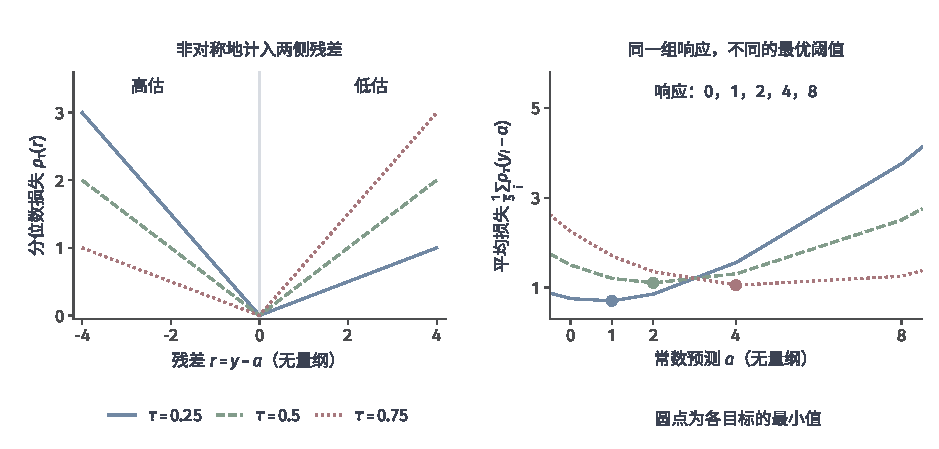
\includegraphics[width=105.412mm]{figures/04-classic-models/00-shared/matplotlib/regression-quantile-objective/figure.pdf}
  \caption{分位数损失$\rho_{0.7}(e)$。正残差（低估响应）斜率为$0.7$，负残差（高估响应）斜率为$-0.3$；零点处有折点。损失不关于零对称，因此最小化它得到的是条件分位数而不是条件均值。}
  \label{fig:regression-quantile-objective}
\end{figure}

给定训练得到的系数$(b_\tau,\bm{w}_\tau)$，对新输入$\bm{x}_\star$的预测就是该分位函数本身：$\widehat f_\tau(\bm{x}_\star)=b_\tau+\bm{w}_\tau^{\top}\bm{x}_\star$；输入先按训练折标准化的同一尺度处理。

\subsubsection{参数学习}
\label{sec:regression-quantile-learning}

把每个残差拆成非负的正部与负部$e_i=u_i-v_i$，$u_i,v_i\geq0$，目标变为线性规划
\begin{equation}
  \min_{b,\bm{w},u,v}
  \sum_{i=1}^n[\tau u_i+(1-\tau)v_i],
  \qquad
  y_i-(b+\bm{w}^{\top}\bm{x}_i)=u_i-v_i.
  \label{eq:regression-quantile-lp}
\end{equation}
目标凸、约束线性。pinball损失关于预测$\hat f_i=f_\tau(\bm{x}_i)$的次梯度为$1\{y_i\leq\hat f_i\}-\tau$——高估（$\hat f_i>y_i$）时为$1-\tau$，低估时为$-\tau$，零点落在区间$[-\tau,\,1-\tau]$内；故
\[
  \partial J/\partial w_j=\frac1n\sum_{i=1}^n\bigl(\mathbb 1\{y_i\leq\hat f_i\}-\tau\bigr)\,x_{ij},
  \qquad
  \partial J/\partial b=\frac1n\sum_{i=1}^n\bigl(\mathbb 1\{y_i\leq\hat f_i\}-\tau\bigr).
\]
实际训练不沿这个次梯度下降，而是拆成非负松弛后走线性规划求解：目标凸、约束线性，可用专门的线性规划或内点法求解，停止依据为原始目标与对偶目标（把约束改写成由乘子描述的等价形式）之差，即对偶间隙逼近零。系数在退化情况下可能不唯一。输入先标准化（尺度取自训练折）以改善数值尺度；逐$\tau$独立求解时应检查相邻分位曲线的稳定性。

\subsubsection{理论分析}
\label{sec:regression-quantile-theory}

对固定$\bm{x}$，设$\tau$分位数为$q_\tau(\bm{x})$，把期望损失按积分拆开：
\[
  \mathbb E[\rho_\tau(Y-a)\mid\bm{x}]
  =\tau\int_a^\infty(y-a)\,dF(y\mid\bm{x})
  +(1-\tau)\int_{-\infty}^a(a-y)\,dF(y\mid\bm{x}).
\]
对$a$求导令其为零得$(1-F(a\mid\bm{x}))\tau-F(a\mid\bm{x})(1-\tau)=0$，即$F(a\mid\bm{x})=\tau$，期望损失最小点正是条件分位数。这一结论不依赖正态假设。分布函数平坦或含原子时最优点可能不唯一；表示不足时只得到该函数类的最佳分位数损失逼近，尾部样本不足会影响估计。若噪声与输入独立、分布固定，各分位函数相互平行；若条件方差随输入扩大，高分位与低分位向两侧散开，斜率可以不同。有限样本下经验超越率与$\tau$有离散偏差，小样本或极端$\tau$（如$0.99$）时更明显，样本量不足以支撑极远尾部的估计。

\subsubsection{支持变量选择：稀疏分位数回归}
\label{sec:regression-quantile-sparsity}

变量多而尾部观测有限时，在平均分位数损失上加一范数惩罚$\lambda\lVert\bm{w}\rVert_1$，系数也拆成正负部分后仍可用线性规划，构成稀疏分位数回归；坐标更新沿用软阈值，数据项换成分位损失的次梯度。稀疏分位曲线用于在少量变量上给出分位预测，按对应分位数损失选择强度，并区分尾部预测与变量识别，不能只按均方误差判断稀疏扩展；被选变量在相邻$\tau$之间可能变动，选择稳定性、额外计算成本与惩罚强度的配置都要在训练折内检查。

\subsubsection{支持多个有序分位点}
\label{sec:regression-quantile-ordering}

逐$\tau$独立估计的曲线可能交叉：低水平曲线跑到高水平曲线上方，此时由两线围成的“区间”方向颠倒，无法解释为从低到高的覆盖带。\term{非交叉}（non-crossing）要求对任意$\bm{x}$，$f_{\tau_1}(\bm{x})\leq f_{\tau_2}(\bm{x})$当$\tau_1<\tau_2$。联合估计一组有序分位$\tau_1<\cdots<\tau_m$，把各分位损失求和，并对相邻函数加入序约束$f_{\tau_{j+1}}(\bm{x})-f_{\tau_j}(\bm{x})\geq0$，构成带不等式约束的凸规划；另一条路线是先独立求解再对预测值重排序，但重排序改变了单条曲线的局部估计。这只保证指定输入集上的线性顺序，不等于全域非交叉，也不等于完整分布；理论上条件分布扩散越大，相邻分位函数的自然间距越宽，有限分位点的尾部样本、超越率与区间覆盖都要在训练折内检查。
